\documentclass{article}
\usepackage[utf8]{inputenc}
\usepackage{graphicx}

% change reference style to [1], remove stupid sorting, language changed so date in ddmmyyyy
\usepackage[backend=biber, style=numeric, sorting=none, language=australian]{biblatex}
\addbibresource{References.bib}

\title{Report}
\author{David Saunders (910995)}
\date{April 2020}

\begin{document}
\maketitle

\begin{abstract} 
    Write abstract here. 4 page report!
\end{abstract}

\tableofcontents

\section{Introduction}

Contextualise the machine-learning problem and introduce the
task and the hypothesis. Make sure to include a few references to previous
work. You should demonstrate an awareness of the research-area.

Write section 1 here \cite{torsney2011tuner} and talk about figure \ref{fig:test}.

Image detection is a classic machine learning problem, with hundreds of papers on the topic. 
History of image detection is relatively recent.
Maybe started with the MNIST handwritten digit classification problem.
Is regarded by many as the 'Hello world' of machine learning/CNNs.
One guy on kaggle used a cnn for the first time to great effect.
Other more advanced problems such as image recognition, gesture
    , emotion detection now possible thanks to deeper networks, and convolution's layers.


Maybe touch on the problem some people have of using too advanced method for the task?
Especially with stuff like pretrained CNN specialised for facial recognition used to detect a black or white dot for example.


\begin{figure}[ht]
    \centering
    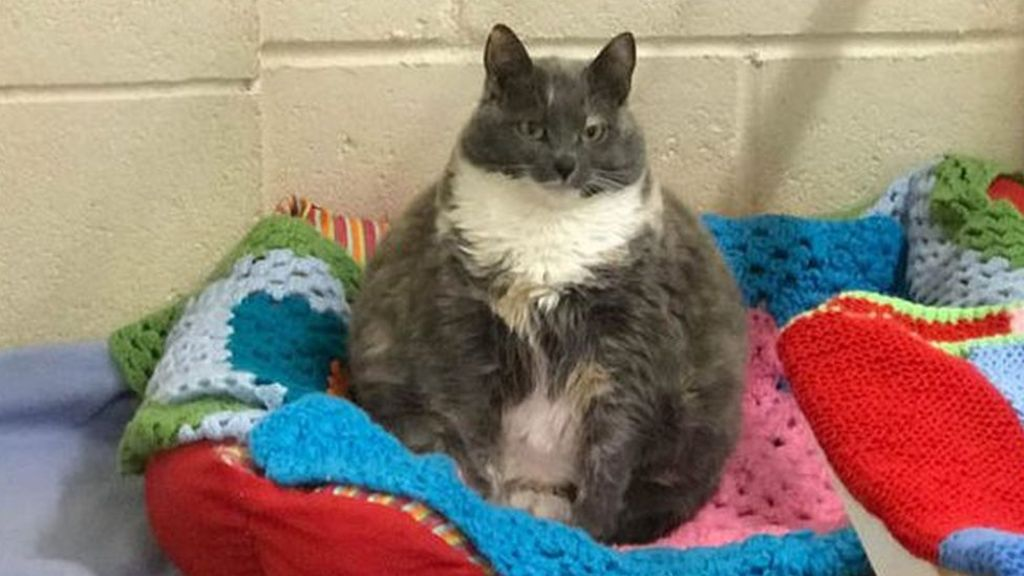
\includegraphics[scale=0.35]{Test.JPG}
    \caption{This will be a figure showcasing some of my work}
    \label{fig:test}
\end{figure}

\section{Methodology}
The model(s) you trained to undertake the task. Any decisions
on hyperparameters must be stated here, including motivation for your
choices where applicable. If the basis of your decision is experimentation
with a number of parameters, then state this.

Decided to use a Convolutionial Neual Network, due to their tried and trusted effectiveness at image detection.
Detecting the red sphere is a trivial use of the technology so accuracy is expected to be very high.
Problem will be with the training data not relating to the real life data where the spheres will be obscured and different sizes from the training.
Problem of training/archived data not matching production is a well known issue (with prediction and stuff) TODO: ref.

All of the architecture of the CNN will be explained in this paragraph and all of the hyperparameter's explained.
Why ADAM, why crossspectromity, LOOK AT LAST YEARS.
(Maybe picture of model summary?, or look at a tool online to visualise)

\section{Results}
Describe, compare and contrast the results you obtained on your
model(s). Any relationships in the data should be outlined and pointed
out here. Only the most important conclusions should be mentioned in
the text. By using tables and confusion-matrices to support the section,
you can avoid describing the results fully.

\section{Discussion and Conclusion}
Restate the task and hypothesis/-ses concisely.
Reiterate the methods used. Describe the outcome of the experiment
and the conclusion that you can draw from these results in respect of the
hypothesis/-ses.

\printbibliography

\end{document}